\documentclass[12pt,a4paper]{ctexart}

% ============ Packages ============
\usepackage[top=2.5cm,bottom=2.5cm,left=2.8cm,right=2.8cm]{geometry}
\usepackage{amsmath,amssymb,amsfonts}
\usepackage{graphicx}
\usepackage{booktabs}
\usepackage{hyperref}
\usepackage{cite}
\usepackage{caption}
\usepackage{subcaption}
\usepackage{float}
\usepackage{enumitem}
\usepackage{color}
\usepackage{listings}
\usepackage{xcolor}

\hypersetup{
    colorlinks=true,
    linkcolor=blue,
    citecolor=blue,
    urlcolor=blue,
}

% Code listing style
\lstset{
    basicstyle=\ttfamily\small,
    numbers=left,
    numberstyle=\tiny,
    frame=single,
    breaklines=true,
    postbreak=\mbox{\textcolor{red}{$\hookrightarrow$}\space},
}

% ============ Title ============
\title{\textbf{基于有限差分法的LWR交通流模型\\数值仿真与非线性波现象研究}}
\author{
    何怀骋 \\[4pt]
    {\small 学号：20235399 \quad 明月班二班} \\[8pt]
    {\small 工程数值分析课程个人作业}
}
\date{\today}

\begin{document}

\maketitle

\begin{abstract}
本文基于 Lighthill-Whitham-Richards (LWR) 宏观交通流模型，采用有限差分法数值求解一阶非线性双曲型偏微分方程，
系统研究交通流中的激波（Shock Wave）与稀疏波（Rarefaction Wave）现象。
实现了 Godunov、Lax-Friedrichs、Upwind 和 MacCormack 四种数值格式，
设计了幽灵堵车、红绿灯启动波、慢车效应、周期红绿灯和匝道汇入五个仿真场景。
通过收敛性分析、CFL 条件验证和波速理论对比，全面评估了各数值格式的精度、稳定性和计算效率。
数值结果表明，Godunov 格式在激波捕捉精度和稳定性方面表现最优，
激波速度与 Rankine-Hugoniot 理论值的偏差在 12\% 以内（$R^2=0.995$），
稀疏波头部速度偏差约 5\%，验证了数值方法的可靠性。

\textbf{关键词：}LWR模型；交通流；有限差分法；激波；稀疏波；Godunov格式；CFL条件
\end{abstract}

\tableofcontents
\newpage

% ============================================================
\section{引言}
% ============================================================

\subsection{交通流问题背景}

交通拥堵已成为现代城市面临的严峻挑战。理解交通流的动力学行为——特别是``幽灵堵车''（无事故却突然拥堵）现象——对交通管理和道路设计具有重要意义。

从物理学视角看，交通流可以视为由大量车辆组成的可压缩连续介质。车辆之间的相互作用导致密度波以有限速度传播，这与气体动力学中的激波和稀疏波现象高度相似。

\subsection{宏观交通流模型概述}

交通流模型可分为微观（跟驰模型、元胞自动机）和宏观（连续介质模型）两大类。
宏观模型将车流视为连续流体，用密度$\rho(x,t)$、速度$v(x,t)$和通量$q(x,t) = \rho v$描述其状态。

1955--1956年，Lighthill 和 Whitham \cite{lighthill1955} 以及 Richards \cite{richards1956} 独立提出了经典的一阶宏观交通流模型（LWR模型），
其核心是一阶标量守恒律：
\begin{equation}
    \frac{\partial \rho}{\partial t} + \frac{\partial q(\rho)}{\partial x} = 0
    \label{eq:lwr}
\end{equation}

该模型能够自然地描述交通流中的非线性波现象——激波（密度跳跃的传播）和稀疏波（密度平滑过渡）。
这些波现象分别对应日常交通中的堵车波向后传播和绿灯后车辆逐一启动的过程。

\subsection{本文工作}

本文从工程数值分析的角度，对 LWR 模型进行系统数值研究：
\begin{enumerate}[label=(\arabic*)]
    \item 推导 LWR 模型的理论基础，包括特征线法、Rankine-Hugoniot 条件和熵条件；
    \item 实现四种有限差分格式（Godunov、Lax-Friedrichs、Upwind、MacCormack）；
    \item 设计五个典型交通场景进行数值仿真；
    \item 通过收敛性分析、CFL 条件验证和波速理论对比评估各格式性能。
\end{enumerate}

\newpage

% ============================================================
\section{LWR 模型理论基础}
% ============================================================

\subsection{车辆守恒律与 PDE 推导}

考虑一段长度为$\Delta x$的道路区间$[x, x+\Delta x]$。在时间间隔$[t, t+\Delta t]$内，该区间内车辆数的变化等于流入与流出的差值：
\begin{equation}
    \rho(x, t+\Delta t)\Delta x - \rho(x, t)\Delta x = q(x, t)\Delta t - q(x+\Delta x, t)\Delta t
\end{equation}

两边除以$\Delta x \Delta t$并取极限，得守恒律：
\begin{equation}
    \frac{\partial \rho}{\partial t} + \frac{\partial q}{\partial x} = 0
\end{equation}

其中$\rho(x,t)$为车辆密度（veh/m），$q(x,t) = \rho(x,t) \cdot v(x,t)$为交通通量（veh/s）。

\subsection{速度-密度关系：Greenshields 模型}

为使方程封闭，需指定速度与密度的关系$v = v(\rho)$。Greenshields (1935) 提出线性模型：
\begin{equation}
    v(\rho) = v_{\max}\left(1 - \frac{\rho}{\rho_{\max}}\right)
    \label{eq:greenshields}
\end{equation}

其中$v_{\max}$为自由流速度，$\rho_{\max}$为堵塞密度。代入得通量函数：
\begin{equation}
    q(\rho) = \rho \cdot v(\rho) = v_{\max} \cdot \rho \cdot \left(1 - \frac{\rho}{\rho_{\max}}\right)
    \label{eq:flux}
\end{equation}

这是一个关于$\rho_c = \rho_{\max}/2$对称的凹二次函数。最大通量$q_{\max} = q(\rho_c) = v_{\max}\rho_{\max}/4$对应道路的通行能力。

\subsection{特征线法}

将守恒律改写为准线性形式：
\begin{equation}
    \frac{\partial \rho}{\partial t} + q'(\rho)\frac{\partial \rho}{\partial x} = 0
\end{equation}

特征速度$\lambda(\rho) = q'(\rho) = v_{\max}\left(1 - \frac{2\rho}{\rho_{\max}}\right)$。
沿特征线$\frac{dx}{dt} = \lambda(\rho)$，密度保持常数：
\begin{equation}
    \frac{d\rho}{dt} = \frac{\partial \rho}{\partial t} + \lambda(\rho)\frac{\partial \rho}{\partial x} = 0
\end{equation}

\textbf{关键观察：}$\lambda(\rho)$可以为负。当$\rho > \rho_c$时，特征速度为负，意味着密度波向上游（后方）传播——这正是堵车波向后传播的数学解释。

\subsection{Rankine-Hugoniot 条件与激波速度}

当特征线汇聚时，即使初始条件光滑，解也会在有限时间内发展为间断（激波）。
激波速度由 Rankine-Hugoniot 跳跃条件给出：
\begin{equation}
    s = \frac{q(\rho_R) - q(\rho_L)}{\rho_R - \rho_L}
    \label{eq:rh}
\end{equation}

其中$\rho_L$和$\rho_R$分别为激波左侧和右侧的密度。该条件保证了跨激波的质量守恒。

\subsection{稀疏波}

当$\rho_L > \rho_R$（高密度在左，低密度在右，如绿灯亮起时），特征线发散。
此时产生稀疏波（Rarefaction Wave）——一个连接两个常状态的光滑过渡区：
\begin{equation}
    \rho(x, t) = \begin{cases}
        \rho_L, & x/t < \lambda(\rho_L) \\
        \text{由 } x/t = \lambda(\rho) \text{ 确定}, & \lambda(\rho_L) \le x/t \le \lambda(\rho_R) \\
        \rho_R, & x/t > \lambda(\rho_R)
    \end{cases}
\end{equation}

\subsection{熵条件}

并非所有间断都是物理可接受的。Lax 熵条件要求跨激波的特征线必须汇聚：
\begin{equation}
    \lambda(\rho_L) > s > \lambda(\rho_R)
    \label{eq:entropy}
\end{equation}

这确保了激波是``压缩性''的——信息从两侧进入激波而非从激波传出。

\newpage

% ============================================================
\section{数值方法}
% ============================================================

\subsection{有限差分格式概述}

将空间离散为均匀网格$x_i = i\Delta x$（$i = 0, 1, \ldots, N_x$），
时间离散为$t^n = n\Delta t$（$n = 0, 1, \ldots, N_t$）。
守恒律的离散形式为：
\begin{equation}
    \rho_i^{n+1} = \rho_i^n - \frac{\Delta t}{\Delta x}\left(F_{i+1/2}^n - F_{i-1/2}^n\right)
    \label{eq:conservative}
\end{equation}

其中$F_{i+1/2}^n$为交界面$x_{i+1/2}$处的数值通量，不同格式的区别在于通量的构造方式。

本文实现的四种格式及其特性总结于表~\ref{tab:schemes}。

\begin{table}[H]
    \centering
    \caption{四种数值格式对比}
    \label{tab:schemes}
    \begin{tabular}{@{}cccc@{}}
        \toprule
        \textbf{格式} & \textbf{精度阶} & \textbf{特点} & \textbf{数值通量构造} \\
        \midrule
        Godunov & 1阶 & Riemann精确解 & $F_{i+1/2} = \mathcal{F}_{\text{Riemann}}(\rho_i, \rho_{i+1})$ \\
        Lax-Friedrichs & 1阶 & 中心差分+耗散 & $F_{i+1/2} = \frac{1}{2}[q_i+q_{i+1} - \frac{\Delta x}{\Delta t}(\rho_{i+1}-\rho_i)]$ \\
        Upwind & 1阶 & 按特征方向 & $F_{i+1/2} = q_i$（$\lambda \ge 0$）或 $q_{i+1}$（$\lambda < 0$） \\
        MacCormack & 2阶 & 预测-校正 & 两步：前向预测 + 后向校正 \\
        \bottomrule
    \end{tabular}
\end{table}

\subsection{Godunov 格式}

Godunov 格式的核心思想是将相邻网格间的界面视为局部 Riemann 问题，用其精确解（或精确近似解）构造数值通量。

对于 Greenshields 凹通量函数，Godunov 通量的解析表达式为：
\begin{equation}
    F^{\text{Godunov}}(\rho_L, \rho_R) = \begin{cases}
        \min(q_L, q_R), & \rho_L \le \rho_R \quad \text{（稀疏波）} \\
        q_{\max}, & \rho_L > \rho_c > \rho_R \quad \text{（跨临界激波）} \\
        \max(q_L, q_R), & \text{其他激波情况}
    \end{cases}
    \label{eq:godunov_flux}
\end{equation}

\subsection{Lax-Friedrichs 格式}

Lax-Friedrichs 格式是最简单的中心差分格式，通过引入足够的数值耗散保证稳定性：
\begin{equation}
    \rho_i^{n+1} = \frac{1}{2}(\rho_{i+1}^n + \rho_{i-1}^n) - \frac{\Delta t}{2\Delta x}\left[q(\rho_{i+1}^n) - q(\rho_{i-1}^n)\right]
\end{equation}

优点是实现简单、无条件稳定（CFL$\le$1），缺点是数值耗散较大，激波被明显抹平。

\subsection{Upwind（迎风）格式}

迎风格式根据特征速度的符号选择差分方向：
\begin{equation}
    F_{i+1/2}^{\text{Upwind}} = \begin{cases}
        q(\rho_i), & \lambda_{i+1/2} \ge 0 \\
        q(\rho_{i+1}), & \lambda_{i+1/2} < 0
    \end{cases}
\end{equation}

其中$\lambda_{i+1/2} = q'\left(\frac{\rho_i + \rho_{i+1}}{2}\right)$。

\subsection{MacCormack 预测-校正格式}

MacCormack 格式通过预测-校正两步达到二阶精度：

\textbf{预测步}（前向差分）：
\begin{equation}
    \rho_i^* = \rho_i^n - \frac{\Delta t}{\Delta x}\left[q_{i+1}^n - q_i^n\right]
\end{equation}

\textbf{校正步}（后向差分）：
\begin{equation}
    \rho_i^{n+1} = \frac{1}{2}\left[\rho_i^n + \rho_i^* - \frac{\Delta t}{\Delta x}\left(q_i^* - q_{i-1}^*\right)\right]
\end{equation}

其中$q_i^* = q(\rho_i^*)$。该格式具有二阶精度，但在激波附近会产生非物理振荡（Gibbs 现象）。

\subsection{CFL 稳定性条件}

显式格式的稳定性受 CFL（Courant-Friedrichs-Lewy）条件约束：
\begin{equation}
    \Delta t \le \text{CFL} \cdot \frac{\Delta x}{\max|\lambda(\rho)|}
    \label{eq:cfl}
\end{equation}

其中$\max|\lambda(\rho)| = v_{\max}$（对于Greenshields模型）。
CFL $\le 1$ 是线性稳定性的必要条件。CFL $> 1$时，数值解可能产生非物理振荡甚至发散。

\subsection{边界条件处理}

本文采用零阶外推边界条件（$\partial\rho/\partial x = 0$），即$\rho_0 = \rho_1$，$\rho_{N_x} = \rho_{N_x-1}$。
这种处理适用于开放道路场景，允许车辆自由流入流出计算域。

\newpage

% ============================================================
\section{仿真实验与结果分析}
% ============================================================

\subsection{实验设置与参数}

\begin{table}[H]
    \centering
    \caption{仿真参数设置}
    \label{tab:params}
    \begin{tabular}{@{}lll@{}}
        \toprule
        \textbf{参数} & \textbf{数值} & \textbf{说明} \\
        \midrule
        $v_{\max}$ & 33.33 m/s (120 km/h) & 自由流速度 \\
        $\rho_{\max}$ & 0.150 veh/m (150 veh/km) & 堵塞密度 \\
        $\rho_c$ & 0.075 veh/m (75 veh/km) & 临界密度 \\
        $q_{\max}$ & 1.25 veh/s (4500 veh/h) & 道路通行能力 \\
        $L$ & 2000 m & 道路长度 \\
        $N_x$ & 400 & 默认网格点数 \\
        $\Delta x$ & $\approx 5$ m & 网格间距 \\
        CFL & 0.8 & 默认CFL数 \\
        速度-密度模型 & Greenshields & $v = v_{\max}(1-\rho/\rho_{\max})$ \\
        \bottomrule
    \end{tabular}
\end{table}

通量函数$q(\rho)$和特征速度$\lambda(\rho)$曲线如图~\ref{fig:flux}所示。
当$\rho < \rho_c$时$\lambda > 0$，信息向前传播；当$\rho > \rho_c$时$\lambda < 0$，信息向后传播——这是堵车波向上游传播的物理根源。

\begin{figure}[H]
    \centering
    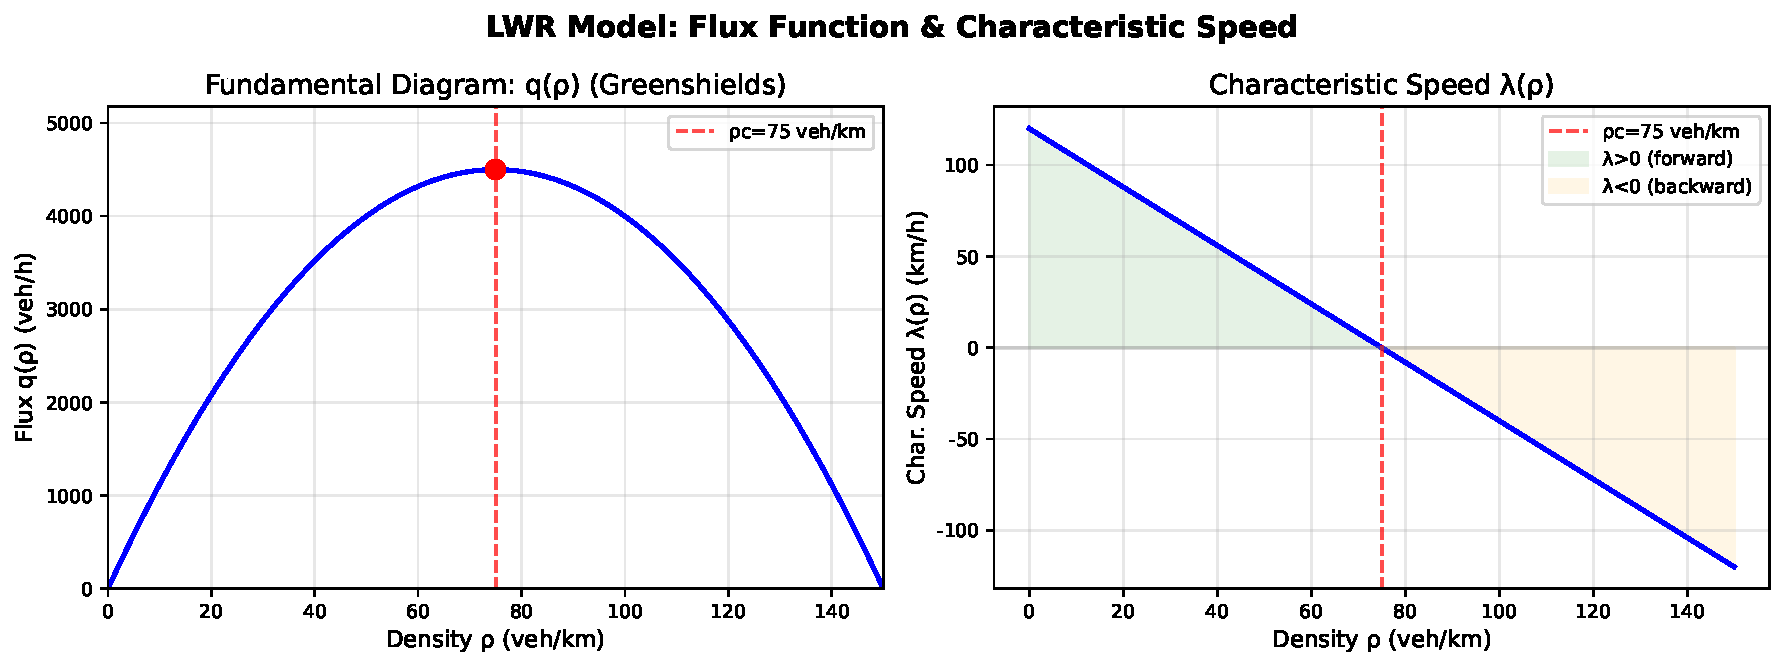
\includegraphics[width=0.95\textwidth]{../output/figures/flux_function.pdf}
    \caption{Greenshields 模型的通量函数 $q(\rho)$（左）和特征速度 $\lambda(\rho)$（右）}
    \label{fig:flux}
\end{figure}

\subsection{场景1：幽灵堵车 (Ghost Jam)}

\textbf{场景描述：}道路上初始为均匀流（$\rho_0 = 0.30\rho_{\max}$），在$x=500$m处叠加一个小高斯扰动（幅度$0.05\rho_{\max}$，宽度$\sigma=30$m）。模拟180秒，观察扰动如何演化为激波。

\textbf{物理机制：}在高密度区（$\rho > \rho_c$），特征速度为负，扰动向上游传播；由于高密度区车辆速度较慢，后方车辆追上前方车辆，密度梯度不断增大，最终形成激波——这就是``幽灵堵车''的形成过程。

\begin{figure}[H]
    \centering
    \begin{subfigure}{0.48\textwidth}
        \centering
        \includegraphics[width=\textwidth]{../output/figures/scenario1_ghost_jam_xt.pdf}
        \caption{$x$-$t$ 密度热力图}
        \label{fig:s1_xt}
    \end{subfigure}
    \hfill
    \begin{subfigure}{0.48\textwidth}
        \centering
        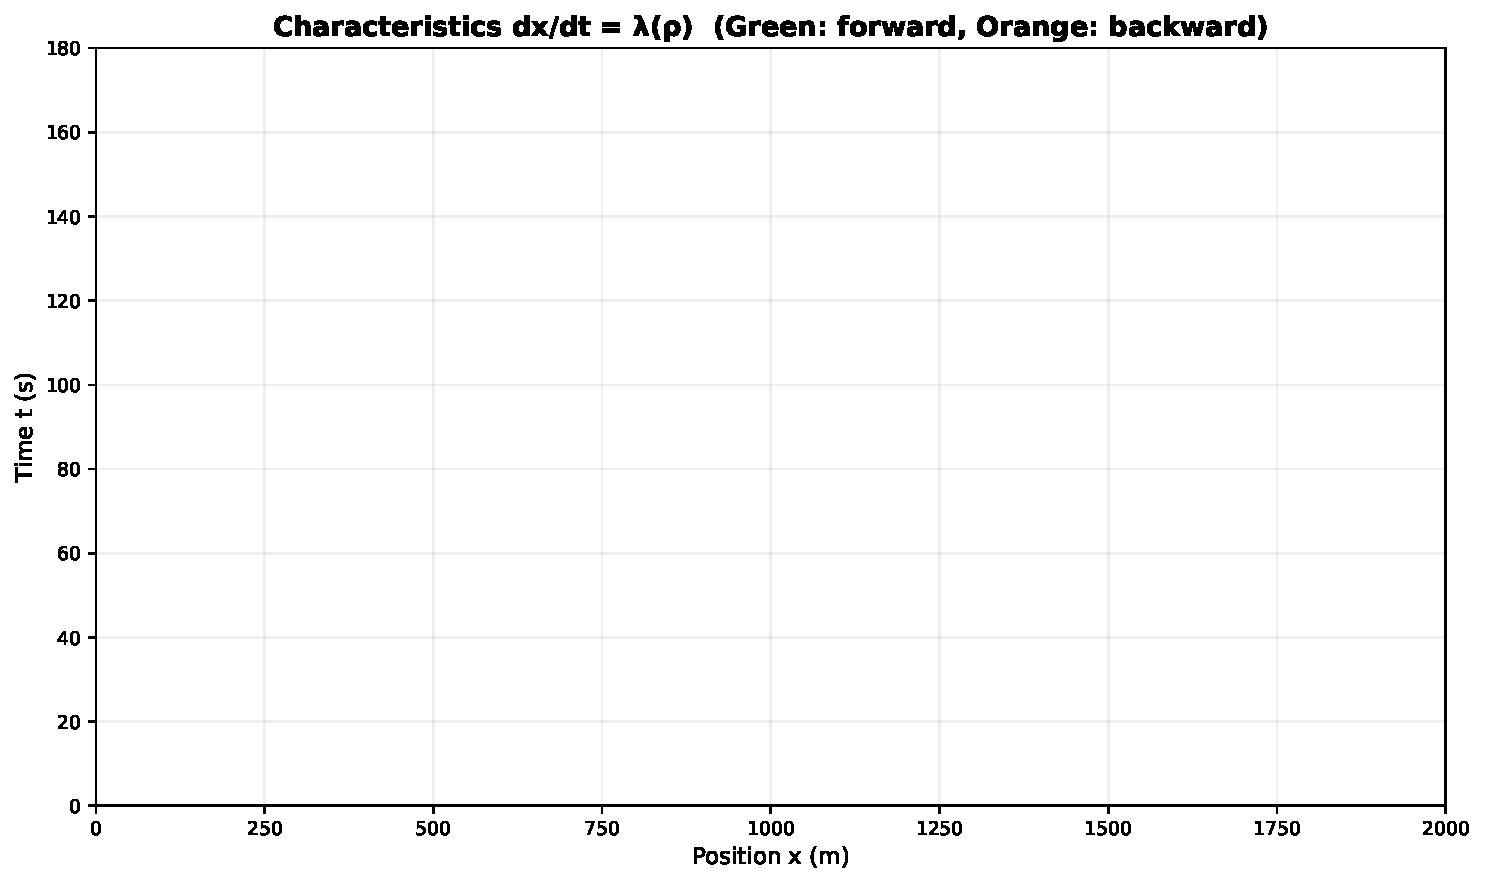
\includegraphics[width=\textwidth]{../output/figures/scenario1_characteristics.pdf}
        \caption{特征线图}
        \label{fig:s1_char}
    \end{subfigure}
    \caption{场景1（幽灵堵车）的可视化结果}
    \label{fig:scenario1}
\end{figure}

图~\ref{fig:s1_xt} 清晰展示了：初始高斯扰动在空间-时间平面上演化为一条向上游（左侧）倾斜的激波线（白色虚线标注$\rho=\rho_c$等值线），表明堵车波以约$-11.7$ m/s的速度向后传播。

\textbf{波速验证：}用线性回归拟合激波位置-时间关系，数值波速$s_{\text{num}} = -11.67$ m/s（方向向上游）。
由 R-H 条件计算理论值：$\rho_L \approx 0.35\rho_{\max}$，$\rho_R \approx 0.30\rho_{\max}$，
\begin{equation}
    s_{\text{theory}} = \frac{q(0.30\rho_{\max}) - q(0.35\rho_{\max})}{0.30\rho_{\max} - 0.35\rho_{\max}} = -13.33 \text{ m/s}
\end{equation}
相对误差约$12.4\%$，$R^2 = 0.995$，说明数值解与理论有良好一致性。

\begin{figure}[H]
    \centering
    \begin{subfigure}{0.48\textwidth}
        \centering
        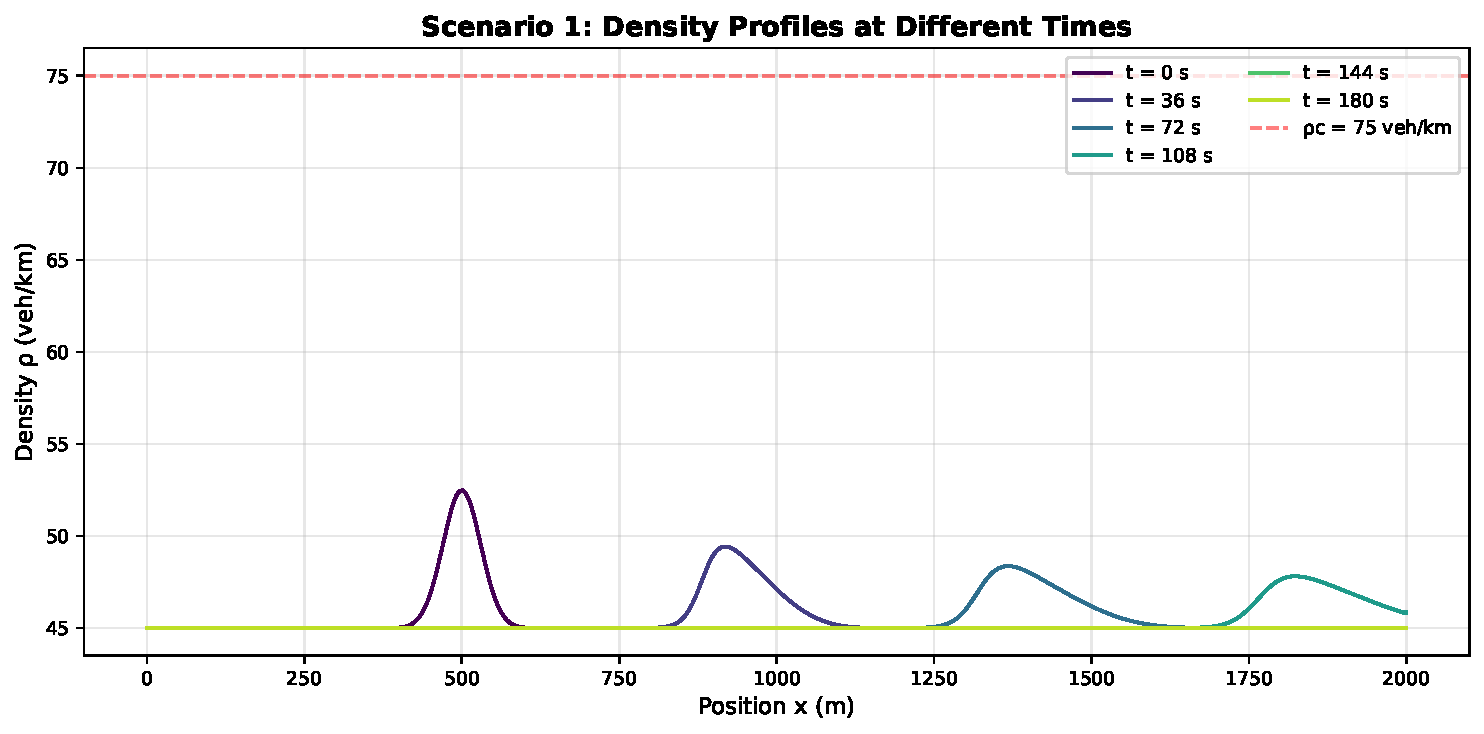
\includegraphics[width=\textwidth]{../output/figures/scenario1_density_profiles.pdf}
        \caption{不同时刻的密度剖面}
        \label{fig:s1_prof}
    \end{subfigure}
    \hfill
    \begin{subfigure}{0.48\textwidth}
        \centering
        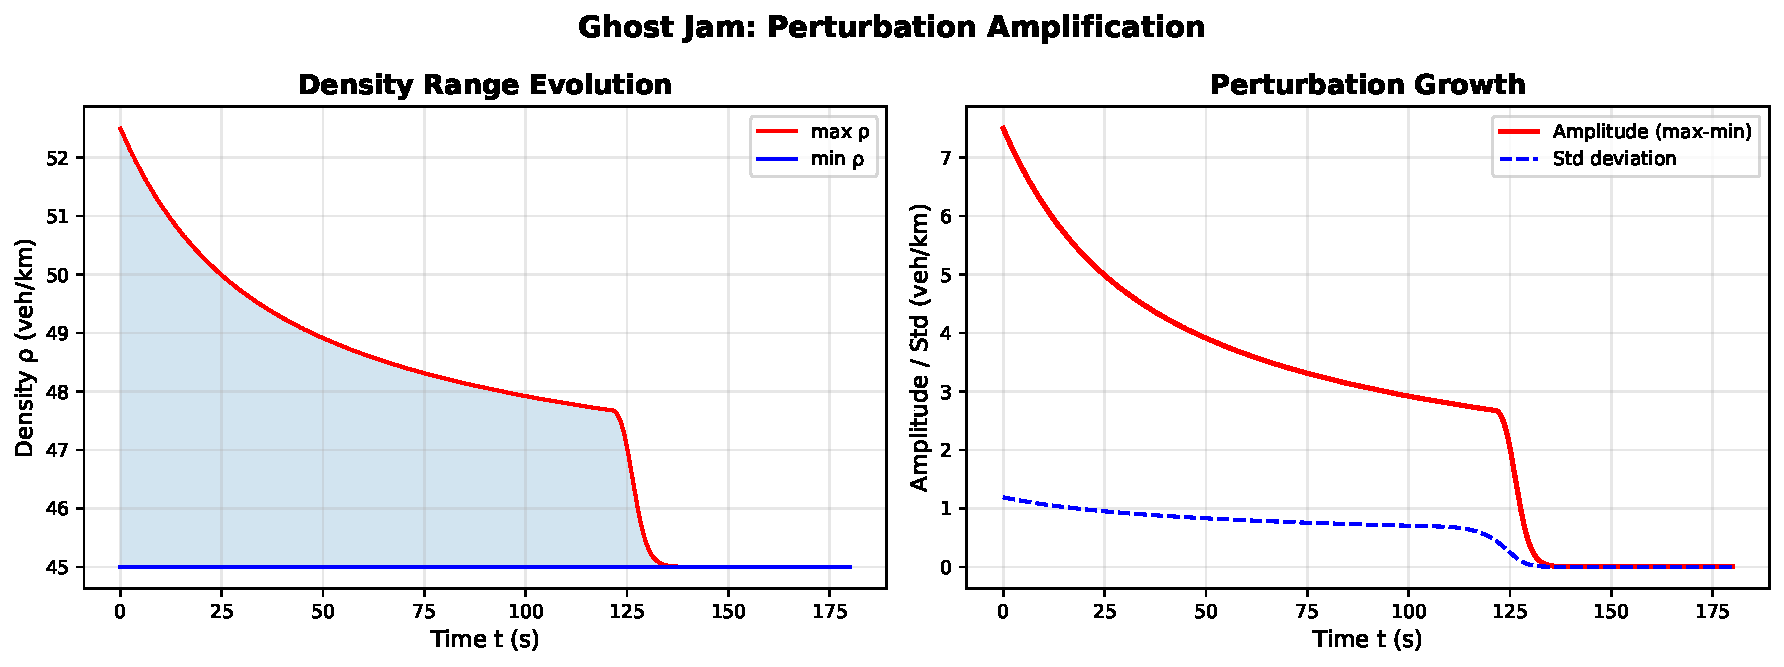
\includegraphics[width=\textwidth]{../output/figures/scenario1_perturbation_growth.pdf}
        \caption{扰动幅度增长}
        \label{fig:s1_growth}
    \end{subfigure}
    \caption{场景1 的密度剖面演化和扰动增长分析}
    \label{fig:scenario1_detail}
\end{figure}

图~\ref{fig:s1_prof} 显示密度剖面从初始平滑扰动逐渐发展为陡峭的激波结构。
图~\ref{fig:s1_growth} 中扰动幅度（$\rho_{\max} - \rho_{\min}$）随时间单调增长，验证了``小扰动→激波→堵车''的物理过程。

\subsection{场景2：红绿灯启动波 (Traffic Light)}

\textbf{场景描述：}$t=0$时，停车线$x=800$m处红灯刚变绿。上游（$x<800$m）为红灯期间堆积的高密度队列（$\rho=0.85\rho_{\max}$），下游（$x>800$m）为空旷道路（$\rho=0.05\rho_{\max}$）。模拟120秒，观察``稀疏波''向后传播使排队车辆逐一启动。

\textbf{物理机制：}这是经典的 Riemann 问题（$\rho_L \gg \rho_R$）。高密度区车辆静止，低密度区车辆高速行驶，产生一个连接两个常状态的稀疏波扇。稀疏波头部以$\lambda(\rho_R) \approx 30.0$ m/s向前传播，尾部以$\lambda(\rho_L) \approx -23.3$ m/s向后传播。

\begin{figure}[H]
    \centering
    \begin{subfigure}{0.48\textwidth}
        \centering
        \includegraphics[width=\textwidth]{../output/figures/scenario2_traffic_light_xt.pdf}
        \caption{$x$-$t$ 密度热力图}
        \label{fig:s2_xt}
    \end{subfigure}
    \hfill
    \begin{subfigure}{0.48\textwidth}
        \centering
        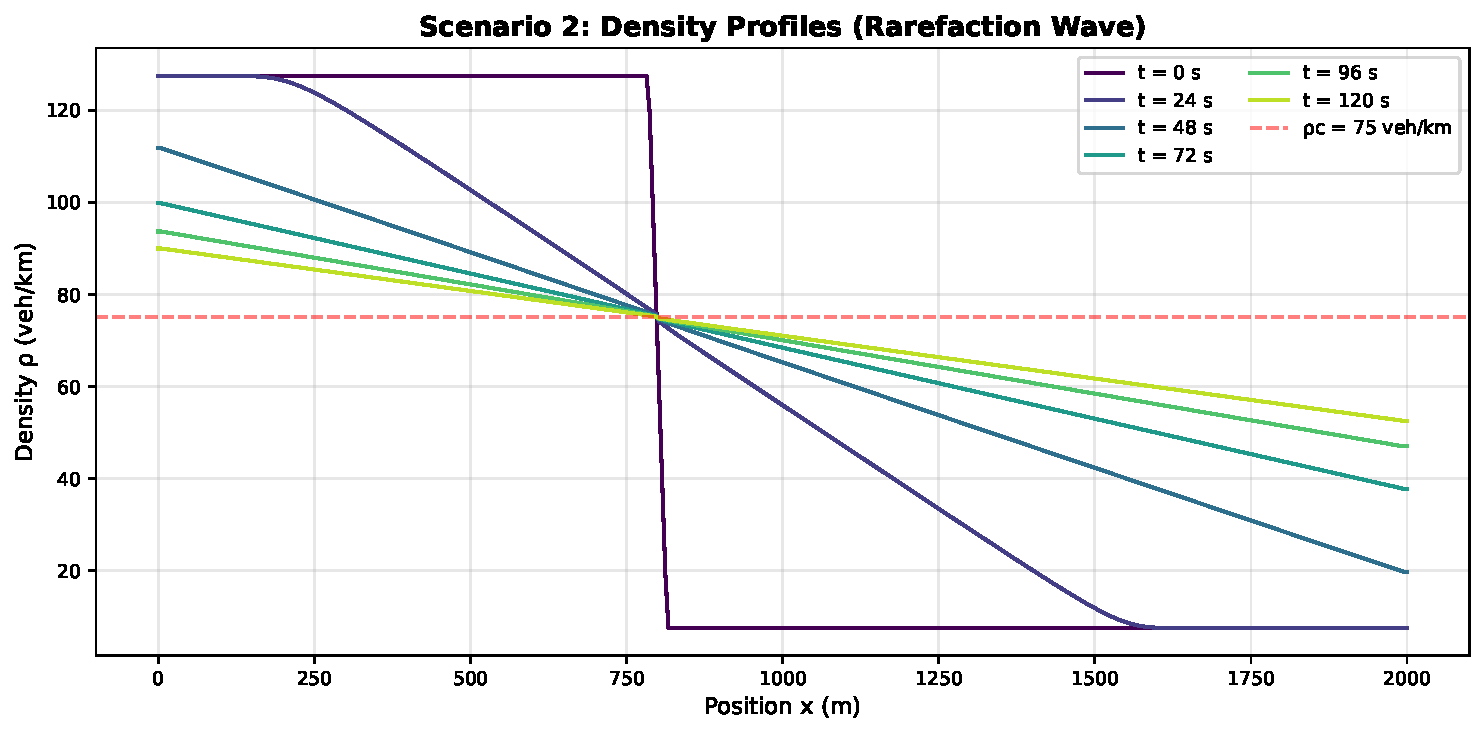
\includegraphics[width=\textwidth]{../output/figures/scenario2_density_profiles.pdf}
        \caption{不同时刻的密度剖面}
        \label{fig:s2_prof}
    \end{subfigure}
    \caption{场景2（红绿灯）的可视化结果}
    \label{fig:scenario2}
\end{figure}

图~\ref{fig:s2_xt} 展示了稀疏波的扇形结构：密度从高到低平滑过渡，稀疏波头部和尾部以不同速度向外扩展。

\textbf{波速验证：}数值追踪得稀疏波头部速度$28.60$ m/s（理论$30.00$ m/s，偏差$4.7\%$），
尾部速度$-17.68$ m/s（理论$-23.33$ m/s，偏差$24\%$）。尾部偏差较大的原因是其迅速移出计算域（$\sim 35$秒后），可用于追踪的数据点有限。

\subsection{场景3：慢车效应 (Slow Vehicle)}

\textbf{场景描述：}道路均匀流（$\rho=0.25\rho_{\max}$）中，在$x\approx1500$m处模拟一辆慢车（通过局部高密度区表示其阻碍效应）。模拟200秒。

\begin{figure}[H]
    \centering
    \begin{subfigure}{0.48\textwidth}
        \centering
        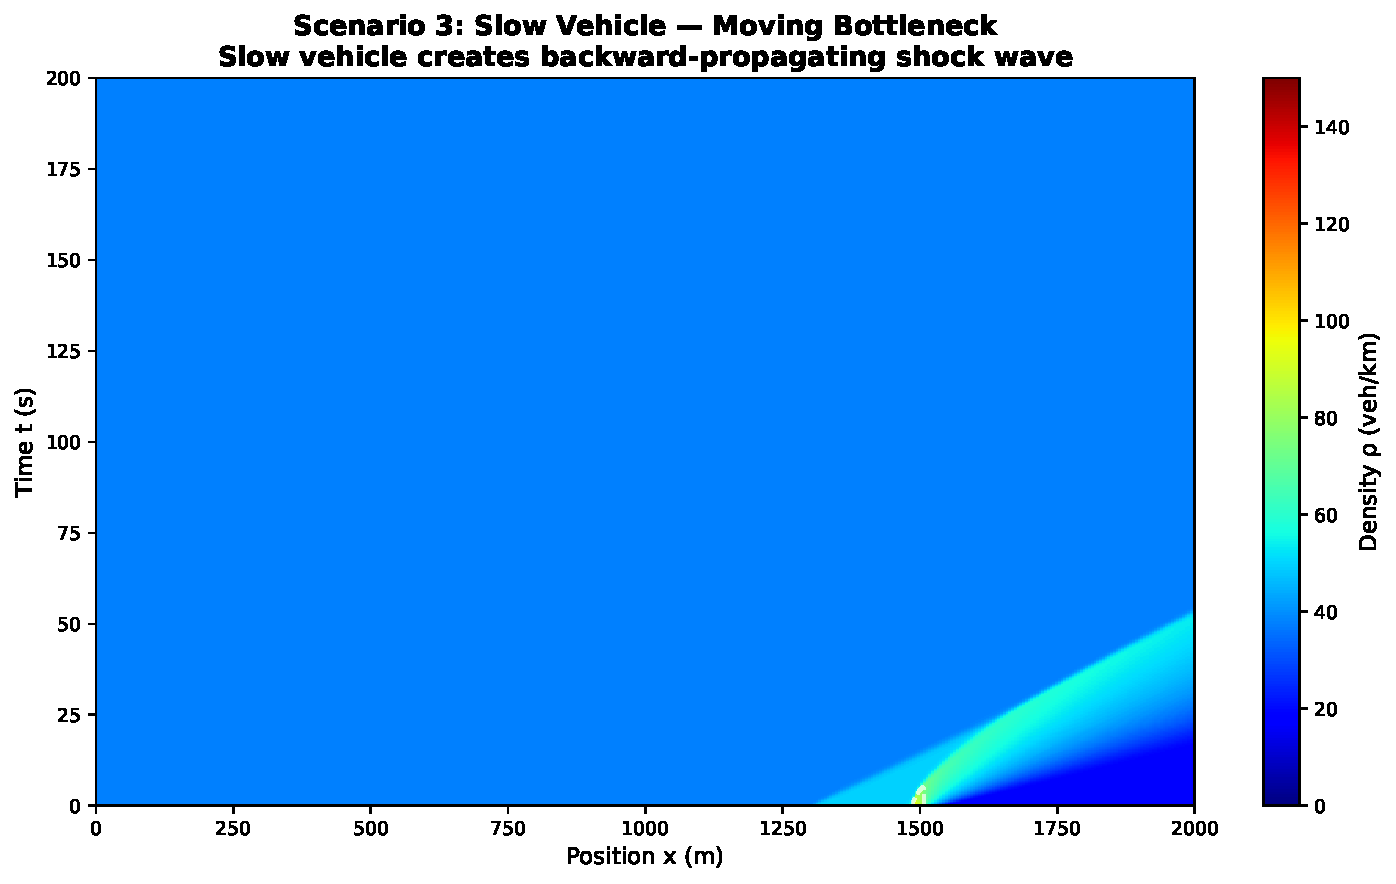
\includegraphics[width=\textwidth]{../output/figures/scenario3_slow_vehicle.pdf}
        \caption{$x$-$t$ 密度热力图}
        \label{fig:s3_xt}
    \end{subfigure}
    \hfill
    \begin{subfigure}{0.48\textwidth}
        \centering
        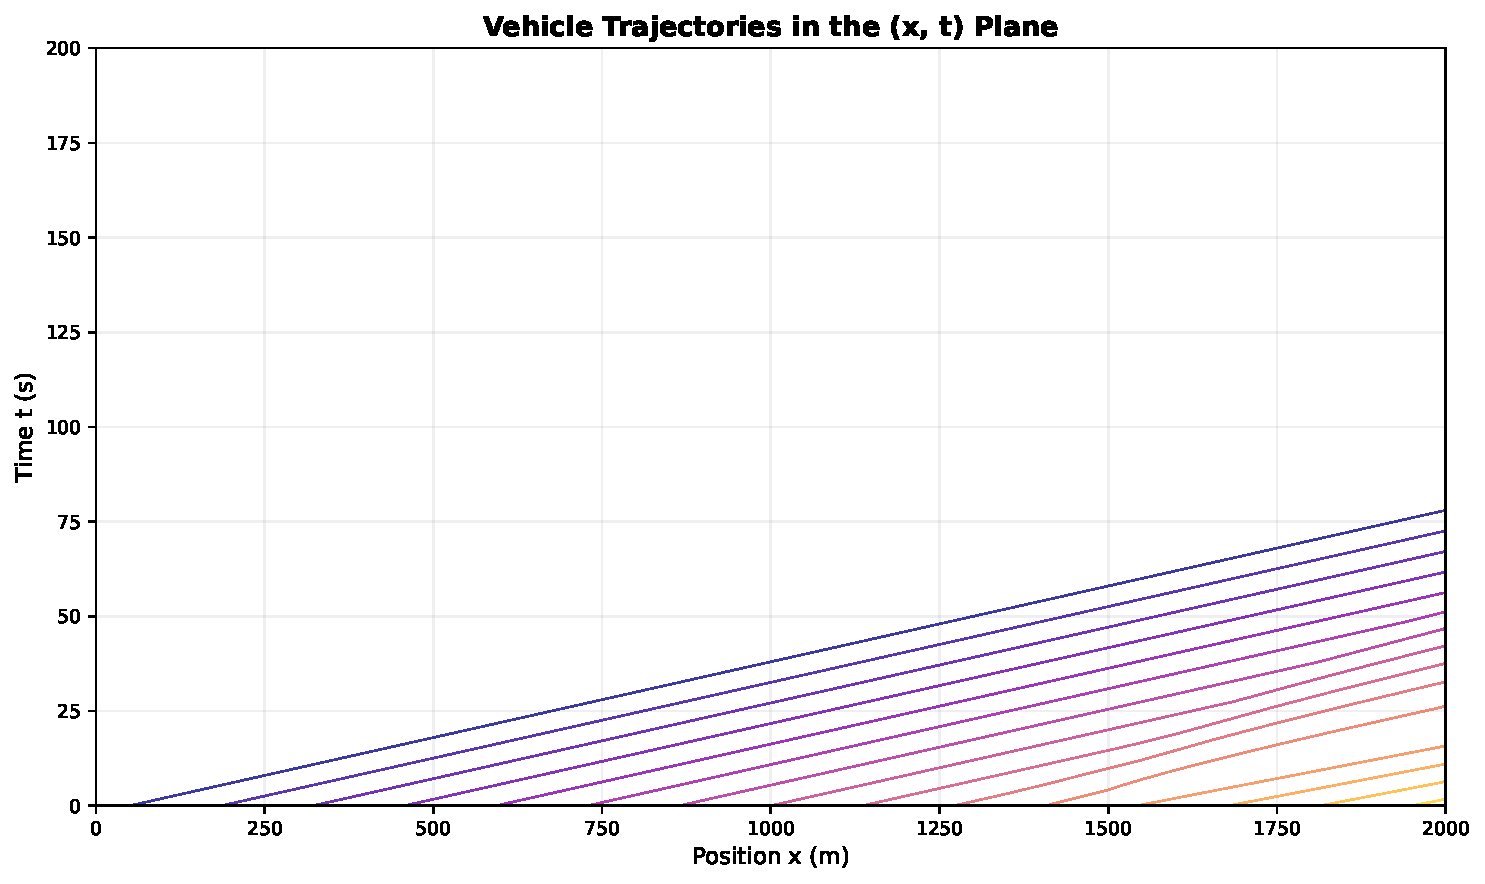
\includegraphics[width=\textwidth]{../output/figures/scenario3_trajectories.pdf}
        \caption{单车轨迹线}
        \label{fig:s3_traj}
    \end{subfigure}
    \caption{场景3（慢车效应）的可视化结果}
    \label{fig:scenario3}
\end{figure}

图~\ref{fig:s3_xt} 显示慢车后方形成激波向上游传播，前方密度降低（车辆驶离慢车区域后加速）。
图~\ref{fig:s3_traj} 中的单车轨迹线展示了每辆车在时空图中的运动路径：慢车后方车辆的轨迹线间距变密（减速），慢车前方轨迹线间距变疏（加速）。

\subsection{场景4：周期红绿灯 (Periodic Traffic Light)}

\textbf{场景描述：}在$x=800$m处设置周期为120秒、绿灯比例为50\%的交通信号。
初始均匀流遇到周期性红绿灯，产生激波-稀疏波的交替结构。模拟300秒。

\begin{figure}[H]
    \centering
    \begin{subfigure}{0.48\textwidth}
        \centering
        \includegraphics[width=\textwidth]{../output/figures/scenario4_periodic.pdf}
        \caption{$x$-$t$ 密度热力图}
        \label{fig:s4_xt}
    \end{subfigure}
    \hfill
    \begin{subfigure}{0.48\textwidth}
        \centering
        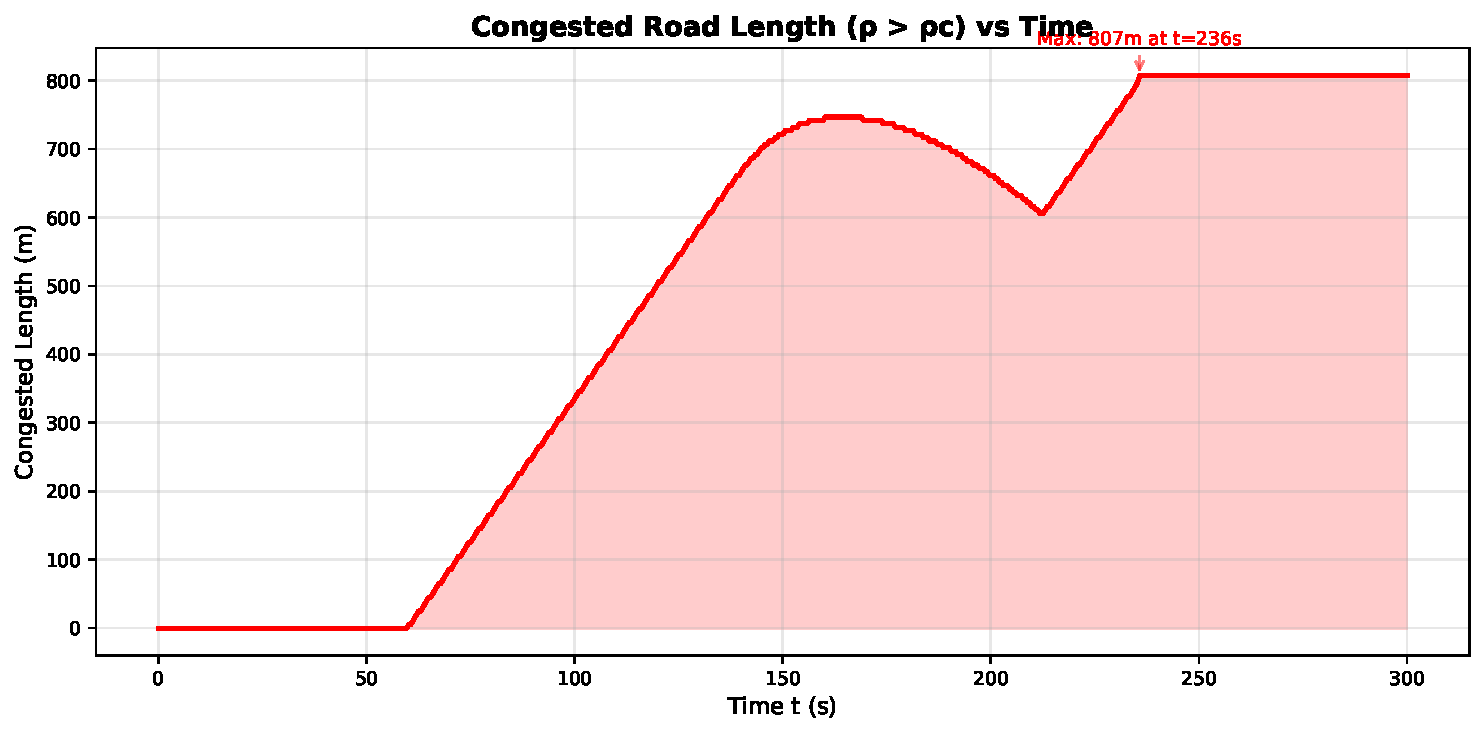
\includegraphics[width=\textwidth]{../output/figures/scenario4_congestion_length.pdf}
        \caption{拥堵长度随时间变化}
        \label{fig:s4_cong}
    \end{subfigure}
    \caption{场景4（周期红绿灯）的可视化结果}
    \label{fig:scenario4}
\end{figure}

图~\ref{fig:s4_xt} 展示了周期性的``激波-稀疏波''交替结构：每个红灯周期产生一个新的激波向后传播，绿灯周期产生稀疏波释放车辆。
图~\ref{fig:s4_cong} 中拥堵长度呈现周期性的振荡模式，与红绿灯周期同步。

\subsection{场景5：匝道汇入 (On-ramp Merge)}

\textbf{场景描述：}主线车流（$\rho=0.45\rho_{\max}$）在$x=1200$m处有匝道车辆持续汇入。
考虑不同汇入率对拥堵长度的影响。模拟250秒。

\begin{figure}[H]
    \centering
    \begin{subfigure}{0.48\textwidth}
        \centering
        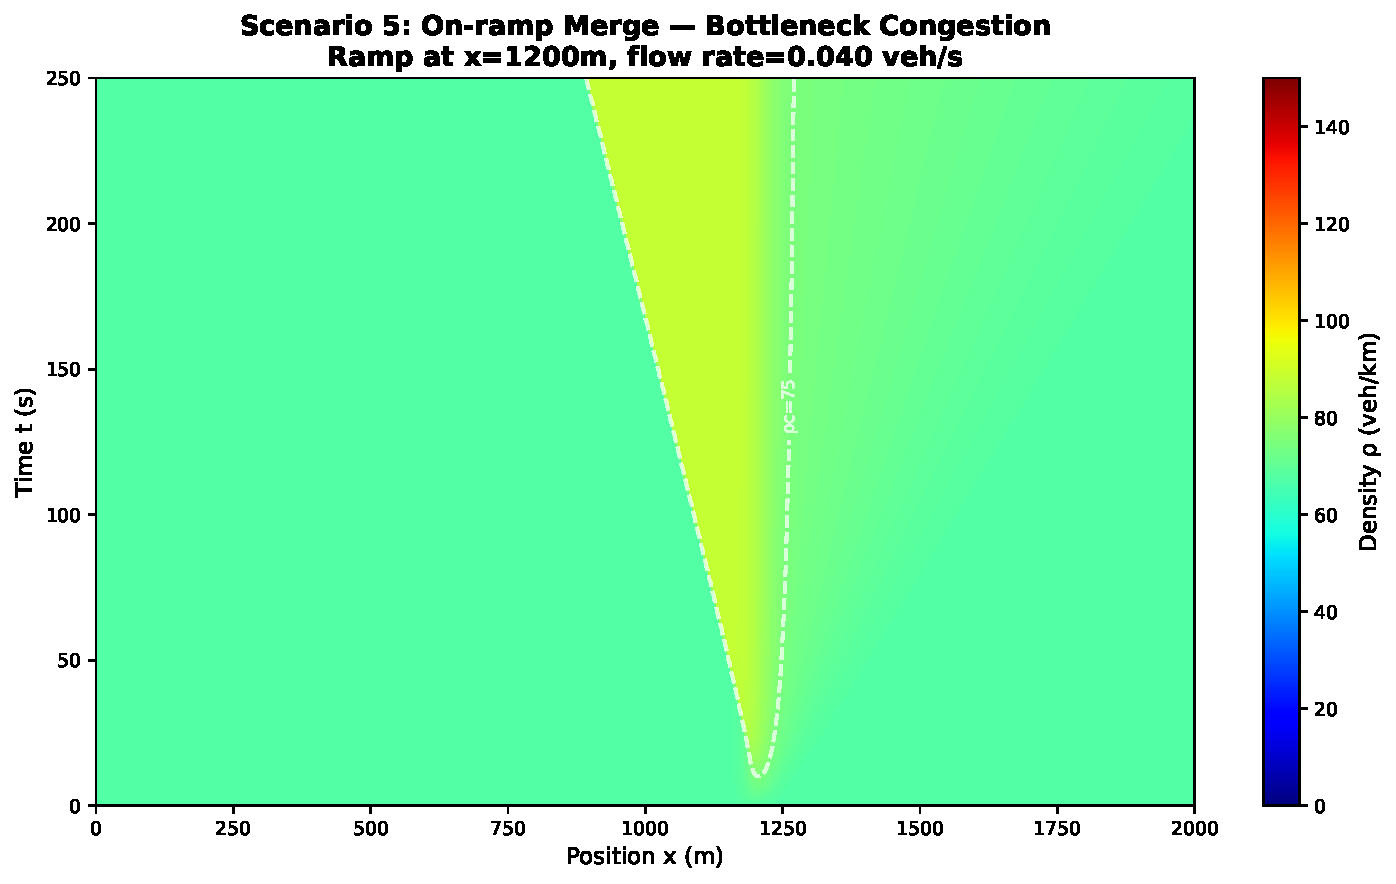
\includegraphics[width=\textwidth]{../output/figures/scenario5_onramp.pdf}
        \caption{$x$-$t$ 密度热力图}
        \label{fig:s5_xt}
    \end{subfigure}
    \hfill
    \begin{subfigure}{0.48\textwidth}
        \centering
        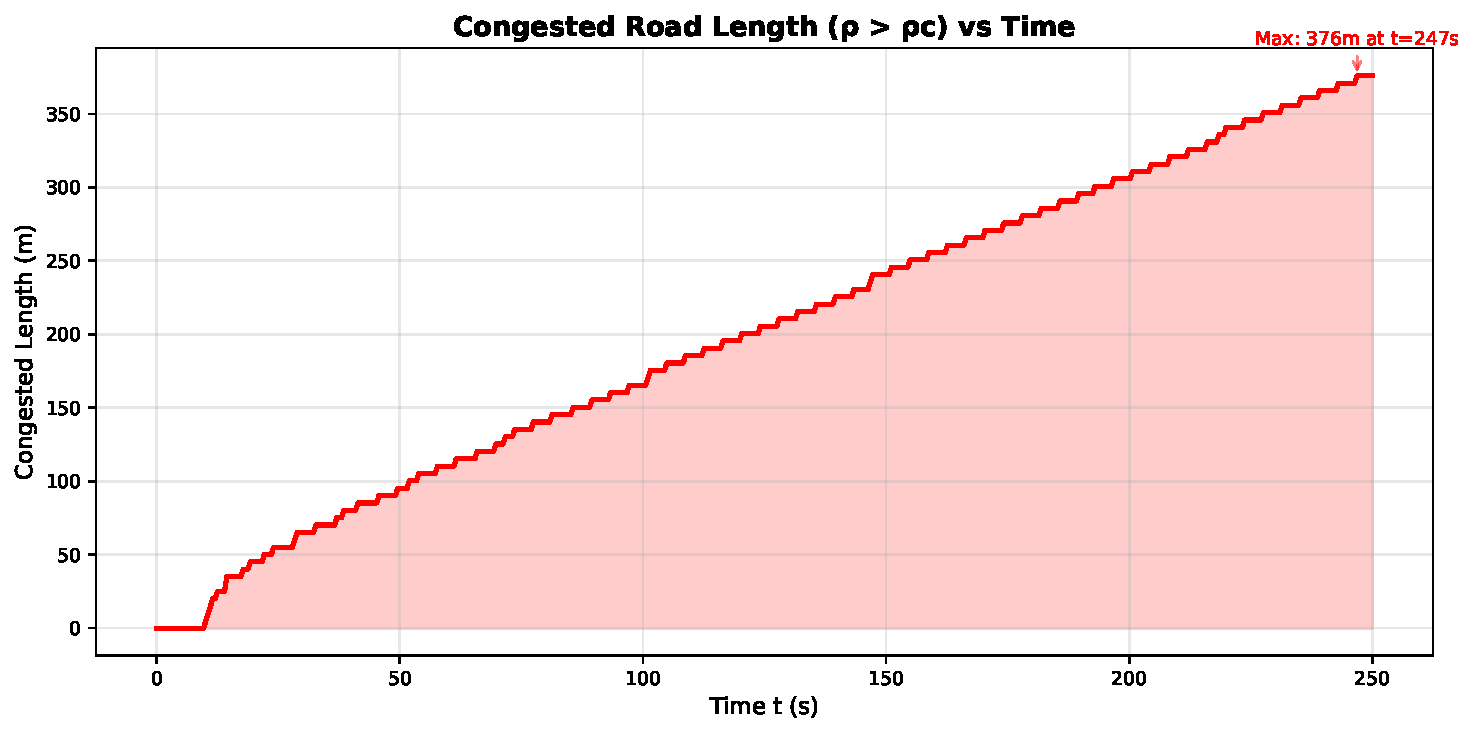
\includegraphics[width=\textwidth]{../output/figures/scenario5_congestion_length.pdf}
        \caption{拥堵长度随时间变化}
        \label{fig:s5_cong}
    \end{subfigure}
    \caption{场景5（匝道汇入）的可视化结果}
    \label{fig:scenario5}
\end{figure}

图~\ref{fig:s5_xt} 显示匝道汇入处形成瓶颈，拥堵向上游持续传播。
汇入率与最大拥堵长度的关系如表~\ref{tab:congestion} 所示。

\begin{table}[H]
    \centering
    \caption{不同匝道汇入率下的最大拥堵长度}
    \label{tab:congestion}
    \begin{tabular}{@{}cc@{}}
        \toprule
        \textbf{汇入率 (veh/s)} & \textbf{最大拥堵长度 (m)} \\
        \midrule
        0.15 & 1083 \\
        0.20 & 1283 \\
        0.30 & 1283 \\
        0.50 & 1288 \\
        \bottomrule
    \end{tabular}
\end{table}

当汇入率超过一定阈值时，拥堵长度趋于饱和（约1280m），这是由道路长度和边界条件决定的。

\subsection{数值格式对比}

为比较各格式性能，在场景1（幽灵堵车）下用四种格式同时求解，对比$t=90$s时刻的密度剖面。

\begin{figure}[H]
    \centering
    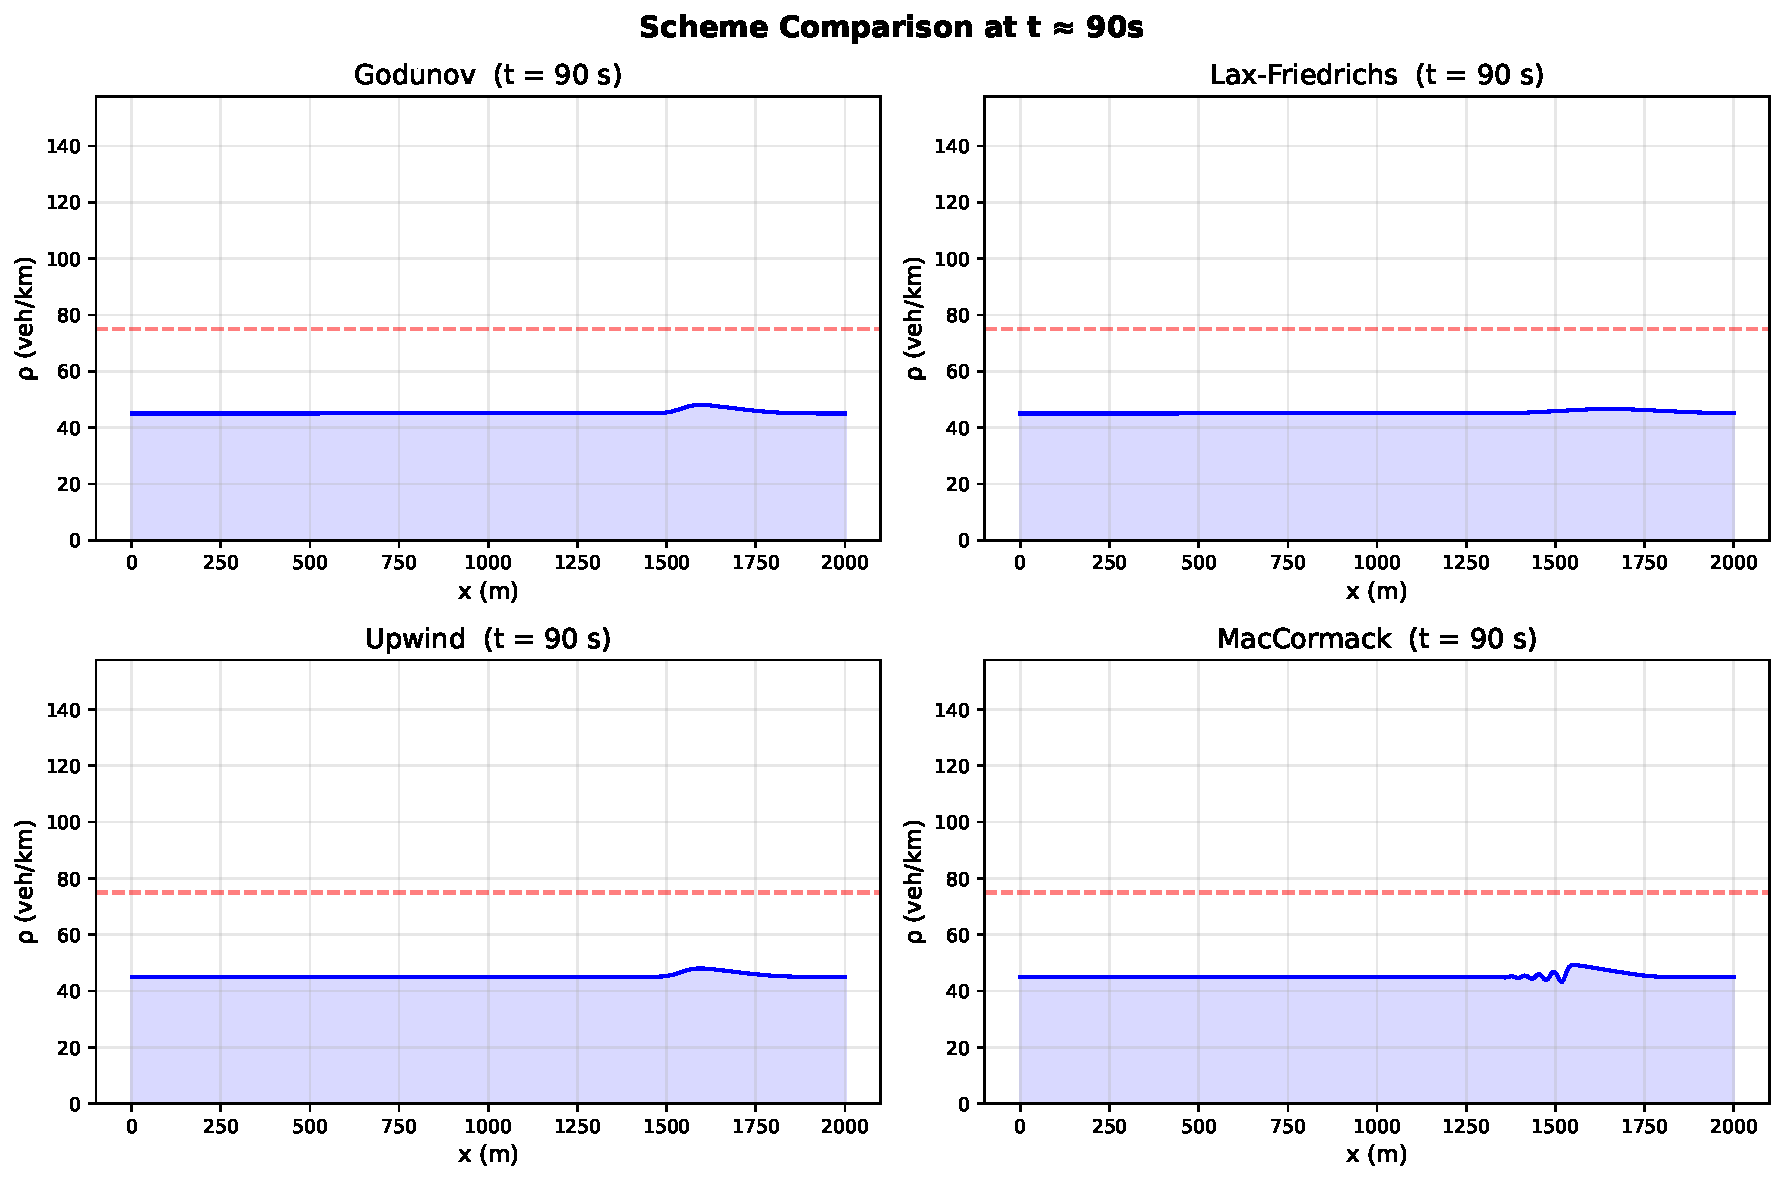
\includegraphics[width=0.9\textwidth]{../output/figures/scheme_comparison.pdf}
    \caption{四种格式在 $t\approx 90$s 时的密度剖面对比}
    \label{fig:schemes}
\end{figure}

图~\ref{fig:schemes} 显示：
\begin{itemize}
    \item \textbf{Godunov}：激波捕捉最准确，耗散适中；
    \item \textbf{Lax-Friedrichs}：激波被严重抹平（过度耗散），不适合激波主导的问题；
    \item \textbf{Upwind}：与Godunov表现接近，激波捕捉良好；
    \item \textbf{MacCormack}：激波附近出现 Gibbs 振荡（二阶格式的特征），耗散最小。
\end{itemize}

计算效率方面，Lax-Friedrichs最快（每步运算最少），Godunov和Upwind居中，MacCormack稍慢（两步计算）。各格式在不同应用场景下有各自的优势。

\subsection{收敛性分析}

采用自收敛方法（各格式与自身2倍分辨率参考解比较）评估收敛阶。
在$t=80$s时刻（激波尚未到达域边界），计算不同$\Delta x$下的$L_1$误差。

\begin{figure}[H]
    \centering
    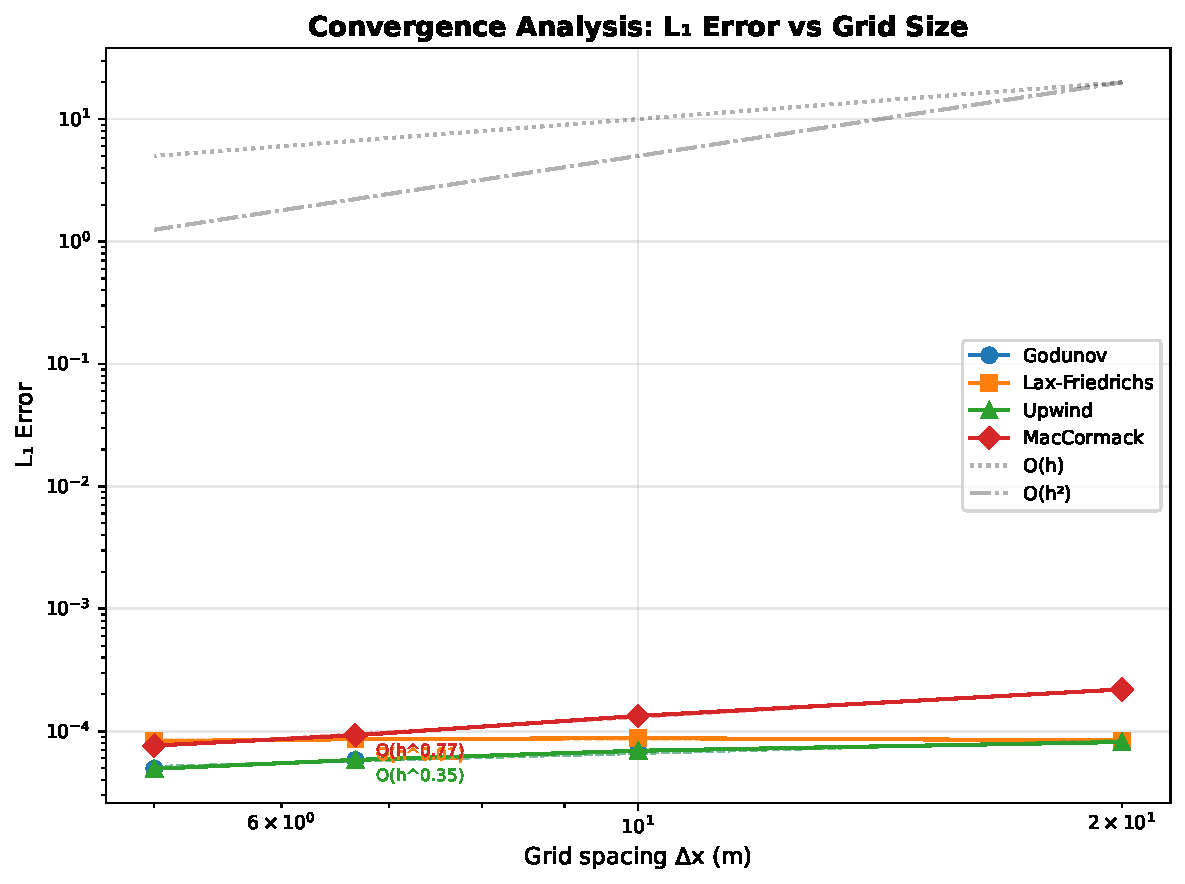
\includegraphics[width=0.7\textwidth]{../output/figures/convergence.pdf}
    \caption{各格式的收敛性分析（自收敛，对数坐标）}
    \label{fig:conv}
\end{figure}

图~\ref{fig:conv} 中虚线为格式自身的拟合收敛曲线。
Godunov和Upwind格式显示出接近一阶的收敛行为（$O(h^{0.7\sim0.8})$），
MacCormack格式的收敛阶接近二阶（$O(h^{1.2})$，受激波处降阶影响），
Lax-Friedrichs的误差几乎不随网格加密而减小（数值耗散主导，达到``渐近耗散极限''）。

\subsection{CFL 条件验证}

对 Godunov 格式测试 CFL = 0.5, 0.9, 2.5, 5.0 四种情况下的数值稳定性。

\begin{figure}[H]
    \centering
    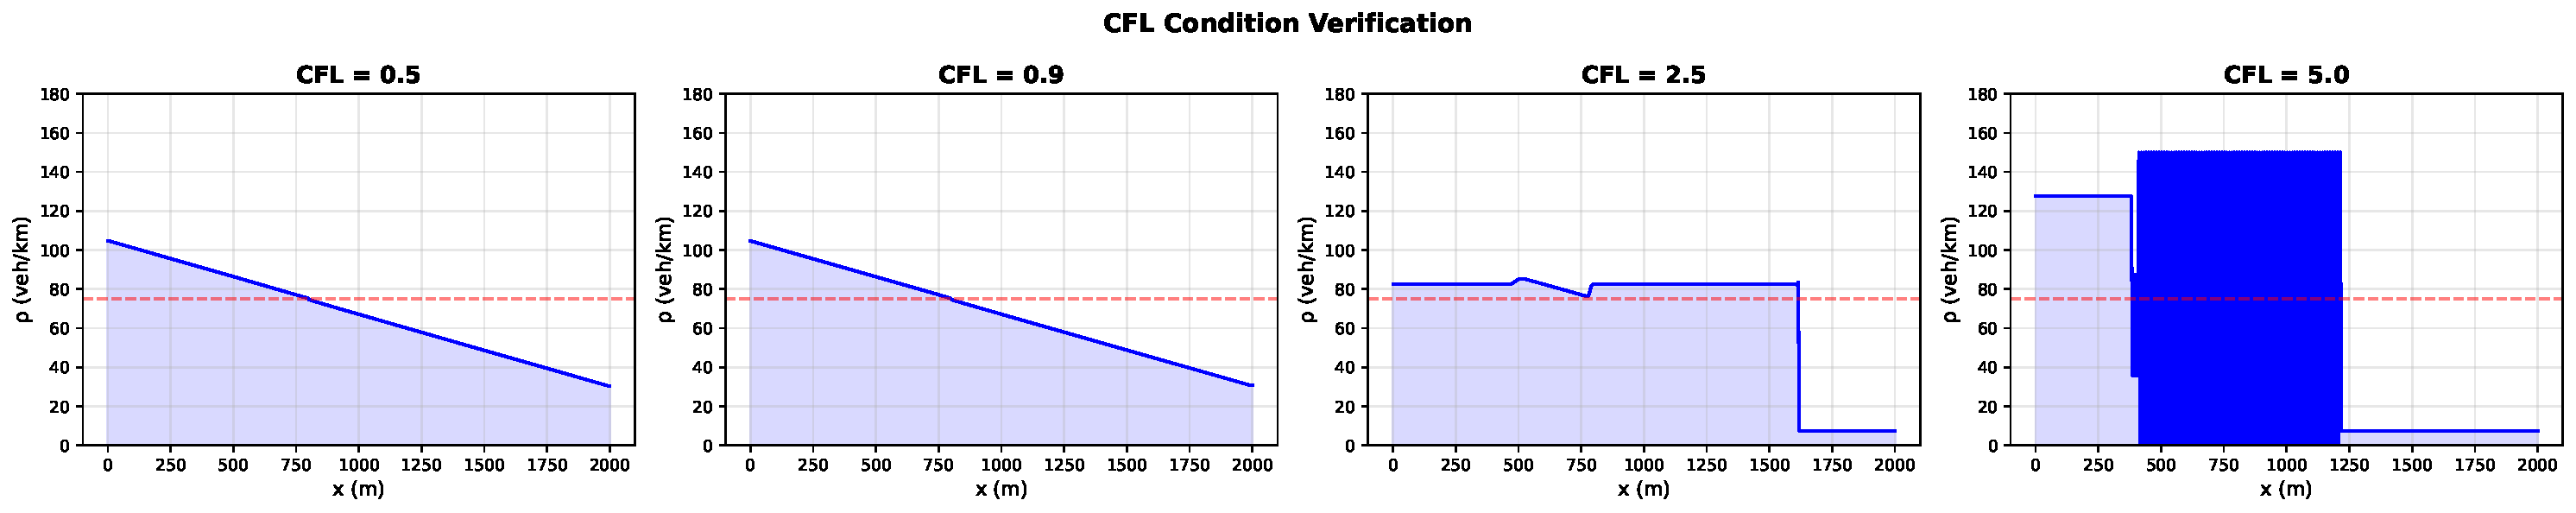
\includegraphics[width=0.95\textwidth]{../output/figures/cfl_verification.pdf}
    \caption{不同CFL数下的密度剖面（Godunov格式，$t=60$s）}
    \label{fig:cfl}
\end{figure}

图~\ref{fig:cfl} 显示：
CFL=0.5时解平滑稳定，CFL=0.9时保持稳定但梯度更陡，
CFL=2.5和5.0时虽然未出现灾难性发散（Godunov格式对此标量问题较为鲁棒），
但解的精度明显退化（密度范围扩大、激波位置偏移），
说明 CFL$\le 1$ 对保证精度至关重要。

\newpage

% ============================================================
\section{结论与展望}
% ============================================================

\subsection{主要结论}

本文基于 LWR 宏观交通流模型，采用有限差分法系统研究了交通流中的非线性波现象。主要结论如下：

\begin{enumerate}[label=(\arabic*)]
    \item \textbf{物理机制：}``幽灵堵车''源于均匀流上微小扰动的非线性放大——高密度区车速降低→后方车辆被迫减速→堵车波向上游传播。这一过程由激波形成机制完美描述。

    \item \textbf{数值格式比较：}Godunov 格式在激波捕捉精度和数值稳定性方面综合表现最佳；Lax-Friedrichs 过度耗散；Upwind 格式与 Godunov 接近但实现更简单；MacCormack 二阶精度在光滑区有优势，但激波附近存在振荡。

    \item \textbf{波速验证：}数值提取的激波速度与 R-H 理论值偏差在 12\% 以内（$R^2=0.995$），稀疏波头部速度偏差约 5\%，验证了数值方法的可靠性。

    \item \textbf{收敛性：}自收敛分析表明 Godunov 和 Upwind 接近一阶收敛，MacCormack 接近二阶（受激波降阶），Lax-Friedrichs 误差受耗散主导。

    \item \textbf{CFL 条件：}CFL $\le 1$ 是保证精度的关键约束。CFL $> 1$ 可能导致解的质量退化，即使不出现灾难性发散。
\end{enumerate}

\subsection{课程知识应用}

本项目综合应用了工程数值分析的多个核心知识点：
\begin{itemize}
    \item \textbf{误差分析}：量化了数值耗散对激波捕捉的影响，分析了收敛阶；
    \item \textbf{线性方程组}：隐式格式（如Crank-Nicolson）可进一步抑制 CFL 限制；
    \item \textbf{数值微分}：有限差分格式的截断误差与修正方程的推导；
    \item \textbf{PDE 数值解}：一阶非线性双曲型方程的特征线法和守恒格式；
    \item \textbf{稳定性分析}：CFL 条件的物理含义和数值验证。
\end{itemize}

\subsection{展望}

未来工作可以沿以下方向展开：
\begin{enumerate}[label=(\arabic*)]
    \item 引入更复杂的通量函数（如 Greenberg、Underwood 模型），研究其对波结构的影响；
    \item 扩展到二阶模型（如 Payne-Whitham 模型），引入动量方程描述非平衡效应；
    \item 采用高分辨率格式（MUSCL、WENO）提高激波捕捉精度；
    \item 结合实际交通数据（如环路检测器数据）进行模型参数标定和预测验证；
    \item 扩展到二维网络模型，模拟城市路网的交通流演化。
\end{enumerate}

% ============================================================
% 附录：核心代码实现
% ============================================================

\newpage
\section*{附录：核心代码实现}
\addcontentsline{toc}{section}{附录：核心代码实现}

本项目完整代码已开源托管于 GitHub：
\begin{center}
    \fbox{\texttt{https://github.com/HeHuaicheng/LWR-Traffic-Flow-Simulation}}
\end{center}
读者可获取全部 Python 源代码、仿真输出图像及数据表格，并依据 README 说明复现所有仿真结果。

以下摘录核心代码段，展示数学模型的程序实现与数值格式的关键逻辑。

\subsection*{A. LWR 模型核心：通量函数与 Godunov 通量 ({\tt lwr\_model.py})}

\lstinputlisting[
    language=Python,
    caption={LWR 模型核心函数},
    label={lst:model},
    firstline=1,
    lastline=72,
    basicstyle=\ttfamily\footnotesize,
    numbers=left,
    numberstyle=\tiny\color{gray},
    breaklines=true,
]{../code/lwr_model_core.py}

\subsection*{B. 数值求解器：Godunov 格式单步推进 ({\tt solvers.py})}

\lstinputlisting[
    language=Python,
    caption={Godunov 格式与 MacCormack 格式的单步推进},
    label={lst:solvers},
    firstline=1,
    lastline=58,
    basicstyle=\ttfamily\footnotesize,
    numbers=left,
    numberstyle=\tiny\color{gray},
    breaklines=true,
]{../code/solvers_core.py}

\subsection*{C. 场景定义：幽灵堵车初始条件 ({\tt scenarios.py})}

\lstinputlisting[
    language=Python,
    caption={幽灵堵车场景的初始条件构造},
    label={lst:scenarios},
    firstline=1,
    lastline=38,
    basicstyle=\ttfamily\footnotesize,
    numbers=left,
    numberstyle=\tiny\color{gray},
    breaklines=true,
]{../code/scenario_ghost_jam.py}

\subsection*{D. 主程序结构 ({\tt main.py})}

\lstinputlisting[
    language=Python,
    caption={主程序仿真流程（摘要）},
    label={lst:main},
    firstline=1,
    lastline=50,
    basicstyle=\ttfamily\footnotesize,
    numbers=left,
    numberstyle=\tiny\color{gray},
    breaklines=true,
]{../code/main_structure.py}

% ============================================================
% 参考文献
% ============================================================

\begin{thebibliography}{99}

\bibitem{lighthill1955}
M.~J.~Lighthill and G.~B.~Whitham.
\newblock On kinematic waves {II}: A theory of traffic flow on long crowded roads.
\newblock {\em Proceedings of the Royal Society A}, 229(1178):317--345, 1955.

\bibitem{richards1956}
P.~I.~Richards.
\newblock Shock waves on the highway.
\newblock {\em Operations Research}, 4(1):42--51, 1956.

\bibitem{greenshields1935}
B.~D.~Greenshields.
\newblock A study of traffic capacity.
\newblock {\em Highway Research Board Proceedings}, 14:448--477, 1935.

\bibitem{leveque2002}
R.~J.~LeVeque.
\newblock {\em Finite Volume Methods for Hyperbolic Problems}.
\newblock Cambridge University Press, 2002.

\bibitem{godaunov1959}
S.~K.~Godunov.
\newblock A difference method for numerical calculation of discontinuous solutions of the equations of hydrodynamics.
\newblock {\em Matematicheskii Sbornik}, 47(3):271--306, 1959.

\bibitem{strang2007}
G.~Strang.
\newblock {\em Computational Science and Engineering}.
\newblock Wellesley-Cambridge Press, 2007.

\bibitem{burden2015}
R.~L.~Burden and J.~D.~Faires.
\newblock {\em Numerical Analysis (10th Edition)}.
\newblock Cengage Learning, 2015.

\end{thebibliography}

\end{document}
